% !TEX encoding = UTF-8 Unicode
\documentclass{sig-alternate}
\usepackage{textcomp}
\usepackage{graphics}
\usepackage[utf8]{inputenc}
\usepackage[T1]{fontenc}

\hyphenation{li-neal co-rrec-ci\'on pro-ble-ma Back-propagation con-si-de-ra}

\begin{document}

\pagenumbering{arabic}

\title{Algoritmos Genéticos}
\subtitle{Sistemas de Inteligencia Artificial - ITBA}

\numberofauthors{3}

\author{
	\alignauthor{Carlos Sessa}\\
	\alignauthor{Lucas Pizzagalli}\\
	\alignauthor{Nicolás Purita}\\	
}

\date{12 de Junio de 2012}

\maketitle

\section{Introducción}

	Se implementó un motor de algoritmo genéticos para obtener los pesos para la red neuronal construida en el Trabajo Práctico número 2.
	La red neuronal resuelve la función que se puede observar en la figura \ref{fig:function}:

	\begin{figure}[!ht]
		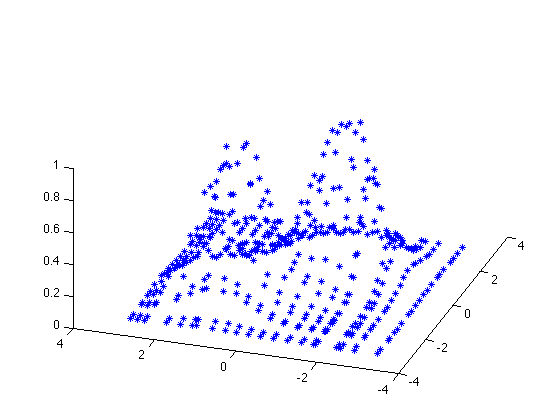
\includegraphics[scale=0.5]{./figures/function.png}
  		\caption{Distribución de puntos dada}
  		\label{fig:function}
	\end{figure}

	En la figura \ref{fig:function} se puede observar que los puntos de la entrada pertenecen al intervalo $[-3.5, 3.5]$ y la salida se encuentra en el intervalo $(0, 1)$.\\
	El algoritmo genético se implementó en \textit{Java} y la red neuronal fue realizada en \textit{Matlab}. Utilizando el \textit{MATLAB Compiler Runtime} se realizan las pruebas pertinentes para verificar el funcionamiento de la red.\\

\section{Nuevo Operador de Cruce}

	\begin{itemize}
		\item \textit{Gene}: Funciona eligiendo las capas que se desean cambiar, a diferencia del clásico que toma un \textit{locus} y a partir del mismo en adelante los cruza.
	\end{itemize}

\section{Desarrollo y Problemas encontrados}

	\subsection{Distintas arquitecturas}

	Mediante el archivo de configuración se puede seleccionar la arquitectura que se desea utilizar para realizar las pruebas. Las arquitecturas elegidas son las siguientes:

	\begin{center}
		\begin{enumerate}
			\item $[30\,20\,10\,1]$
			\item $[10\,10\,1]$
			\item $[10\,1]$
			\item $[10\,10\,10\,10\,1]$
			\item $[40\,20\,1]$
			\item $[10\,10\,10\,1]$
			\item $[5\,10\,20\,1]$
		\end{enumerate}
	\end{center}

	\subsection{Representación del individuo}

	La representación mas óptima del individuo fue representar a toda la red como un vector de números flotantes (Double). Esta representación no se adapta a la representación de la matriz en \textit{MATLAB}, por lo tanto se realiza una transformación del individuo. Esta transformación consiste en cambiar la cadena de Doubles a una matriz y viceversa.

	\subsubsection{Fidelidad del individuo}

	\begin{itemize}
		\item \textbf{Completitud}: Es completa ya que se puede representar todo el dominio del problema. Esto quiere decir que se pueden utilizar todas las cadenas de números para representar la red. 

		\item \textbf{Coherencia}: Representa unicamente el dominio del problema, ya que ninguna representación puede pertenecer al un conjunto fuera del dominio.

		\item \textbf{Uniformidad}: Podemos concluir que esta representación es uniforme ya que es imposible representar dos redes con la misma arquitectura de la misma forma, en caso que esto sucediera esa red es exactamente la misma.	

		\item \textbf{Sencillez}: Es sencilla ya el individuo sabe que cantidad de neuronas que tiene en cada capa por lo tanto dividir un vector es sencillo del mismo modo que transformar una matriz en un vector.

		\item \textbf{Localidad}: Es local esta representación ya que al hacer pequeños cambios sobre la red, instantaneamente cambia la red.
	\end{itemize}
	
\section{Resultados y Conclusiones}

	\subsection{Contexto general}

	Con el fin de obtener resultados comparables entre sí se define un contexto en base para todas las pruebas. Luego en cada prueba se reemplaza el caso base con lo que se desea. A continuación se muestra el contexto base:

	\begin{itemize}
		\item Tamaño de la población es de 52 individuos.
		\item La brecha generacional (\textit{G}) es de 0.5
		\item La arquitectura elegida para realizar las pruebas es la de [10 10 1].
		\item El operador de mutación inicial es \textit{Clásico} con una probabilidad de 0.5 de mutar.
		\item El operador de cruce inicial es \textit{Clásico} con una probabilidad de 1 de cruce.
		\item El operador \textit{Backpropagation} se encuentra desactivado es decir que se ejecute con probabilidad 0.
		\item El método de reemplazo es \textit{Elite}
		\item El método de reemplazo es \textit{Elite} al igual que el de selección
		\item Hay dos condiciones de corte, ya sea por \textit{Máxima cantidad de generaciones} y \textit{Contenido}, donde la última verifica que si en 50 épocas no mejoro mas de un 0.01 el fitness del individuo finaliza su ejecución.
	\end{itemize}

	Debe tenerse en cuenta que el hecho de prefijar algunos parámetros puede hacer que los distintos métodos y operadores a comparar se vean beneficiados o perjudicados por su funcionamiento en conjunto.

	\subsection{Elección del operador de Cruza}

	\subsection{Elección del operador de Mutación}

	\subsection{Utilización de backpropagation}

	\subsection{Elección del operador de Selección y reemplazo}

\end{document}
